\documentclass{beamer}
\usepackage[utf8]{inputenc}
\usepackage{graphicx}
\usepackage{listings}
\usepackage{hyperref}
\hypersetup{
	colorlinks=true,
	linkcolor=blue,
	filecolor=magenta,      
	urlcolor=cyan,
}

\urlstyle{same}

\usepackage{xcolor}

\lstdefinestyle{base}{
	language=C++,
	emptylines=1,
	breaklines=true,
	basicstyle=\ttfamily\color{black},
	moredelim=**[is][\bf\color{red}]{@}{@},
}

\usetheme[]{boxes}
\usecolortheme{seagull}
\addtobeamertemplate{navigation symbols}{}{%
	\usebeamerfont{footline}%
	\usebeamercolor[fg]{footline}%
	\hspace{2em}%
	\insertframenumber/\inserttotalframenumber
}

%\usepackage{french}
\title{Programmation parallèle hybride}
\author{Marc Tajchman}\institute{CEA - DEN/DM2S/STMF/LMES}
\date{10/12/2020}

\begin{document}
\begin{frame}
	\titlepage
\end{frame}

\large
\begin{frame}
	\frametitle{Cas envisagés}

Du fait qu'il y a souvent plusieurs dispositifs matériels (clusters, machines multi-c\oe urs, GPU, etc.) et plusieurs outils logiciels associés, il est intéressant d'essayer de combiner leur utilisation.

\vfill
En fonction de ce qui est disponible sur les machines
\begin{enumerate}
	\item clusters (plus généralement, machines parallèles multi-n\oe uds) : MPI,
	\item processeurs multi-c\oe urs : OpenMP (et autres outils : TBB, std::threads, ...),
	\item accélérateurs de calcul (GPU ou autres) : Cuda, OpenCL,
	\item outils PGAS (``partitionned global addressing system") : pour information (faibles performances),
\end{enumerate}

\vfill
on testera plusieurs combinaisons.
\end{frame}

\begin{frame}
\frametitle{Machines multi-n\oe uds et multi-c\oe urs}

Pour utiliser la puissance de calcul de ce type de machine, on a souvent le choix entre 2 possibilités :
\medskip
\begin{itemize}
	\item {\bf MPI} pour le parallélisme multi-n\oe uds et {\bf MPI} pour le parallélisme multi-c\oe urs (plusieurs processus MPI sur chaque n\oe ud).
\medskip
	\item {\bf MPI} pour le parallélisme multi-n\oe uds et {\bf OpenMP} pour le parallélisme multi-c\oe urs (un processus MPI sur chaque n\oe ud).
\end{itemize}
\vfill

Sur des simulations de taille petite ou moyenne, on préfère souvent le premier choix pour des raisons de simplicité. 

Par contre, sur des simulations de (très) grande taille, le ``tout MPI'' atteint plus rapidement ses limites d'utilisation.
\end{frame}

\begin{frame}
	
\vfill

Avantages/inconvénients du tout MPI:
	
\vfill
\begin{itemize}
	\item[\LARGE $\mathbf\oplus$] programmation MPI n\oe uds-c\oe urs identique à la programmation MPI entre les n\oe uds
	\vfill
	
	\item[\LARGE $\mathbf\oplus$] les librairies MPI sont de mieux en mieux optimisées (en particulier si plieurs processus sont sur le même processeur)
	
\vfill
	\item[\LARGE $\mathbf\ominus$] le nombre de processus MPI augmente plus vite (n° c\oe urs $\times$ n° n\oe uds), les structures internes de MPI, la mémoire utilisée pour les communications aussi (``cellules fant\^omes'', ``halos'')
	\bigskip
	
\bigskip

	\begin{quote}
On atteint actuellement les limites des machines parallèles sur des simulations avec des nombres de processus $> 10^6$.
	\end{quote}
	
\end{itemize}
\vfill
\end{frame}

\begin{frame}


\vfill
	Avantages/inconvénients de la combinaison MPI-OpenMP:
	
\vfill
	\begin{itemize}
		\item[\LARGE $\mathbf\oplus$] les possibilités en nombre de n\oe uds-c\oe urs sont plus importantes
		
\begin{quotation}\noindent%
Le nombre total de processus MPI diminue (un seul processus MPI par n\oe ud de calcul.)
\end{quotation}
	
\vfill
		\item[\LARGE $\mathbf\ominus$] la programmation MPI sur les n\oe uds et OpenMP sur les c\oe urs est plus complexe
	
\vfill
		\item[\LARGE $\mathbf\ominus$] l'amélioration des performances n'est pas toujours évidente surtout pour des nombres de processus petits ou moyens.
	\end{itemize}
	
	\vfill
\end{frame}

\begin{frame}
	Exemples4/MemoireMPI : ressource mémoire utilisée par MPI (MPI\_Init et MPI\_Finalize, seulement, pas d'échange de messages).
	\bigskip
	
	Lire le fichier README.txt pour des instructions
\end{frame}

\begin{frame}
	Combinaison des modèles MPI et OpenMP en modèle hybride MPI-OpenMP:

\begin{center}
	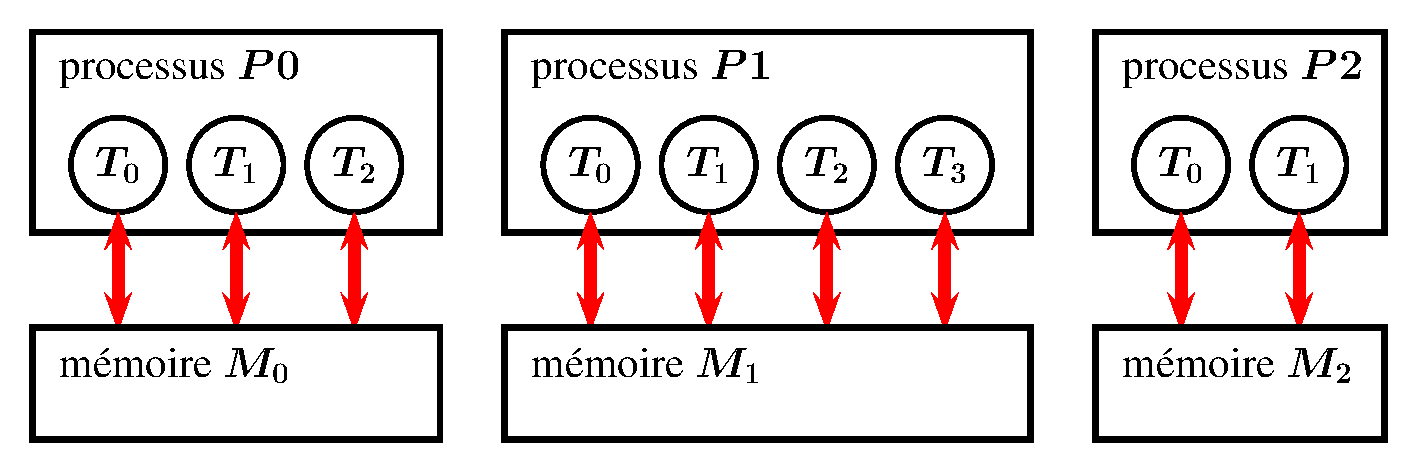
\includegraphics[scale=0.45]{../../Images/modeleHybride}
\end{center}

\begin{itemize}
	\item Les différents processus $P_0$, $P_1$, ... ont chacun leur mémoire locale $M_0$, $M_1$, ....
	\item A l'intérieur de chaque processus $P_i$, un ou plusieurs threads travaillent avec la mémoire locale $M_i$.
	\item Tous les threads peuvent \textsl{a priori} envoyer et recevoir des messages MPI.
\end{itemize}
\end{frame}

\begin{frame}
	Exemple sur 2 processus, chacun avec plusieurs threads
	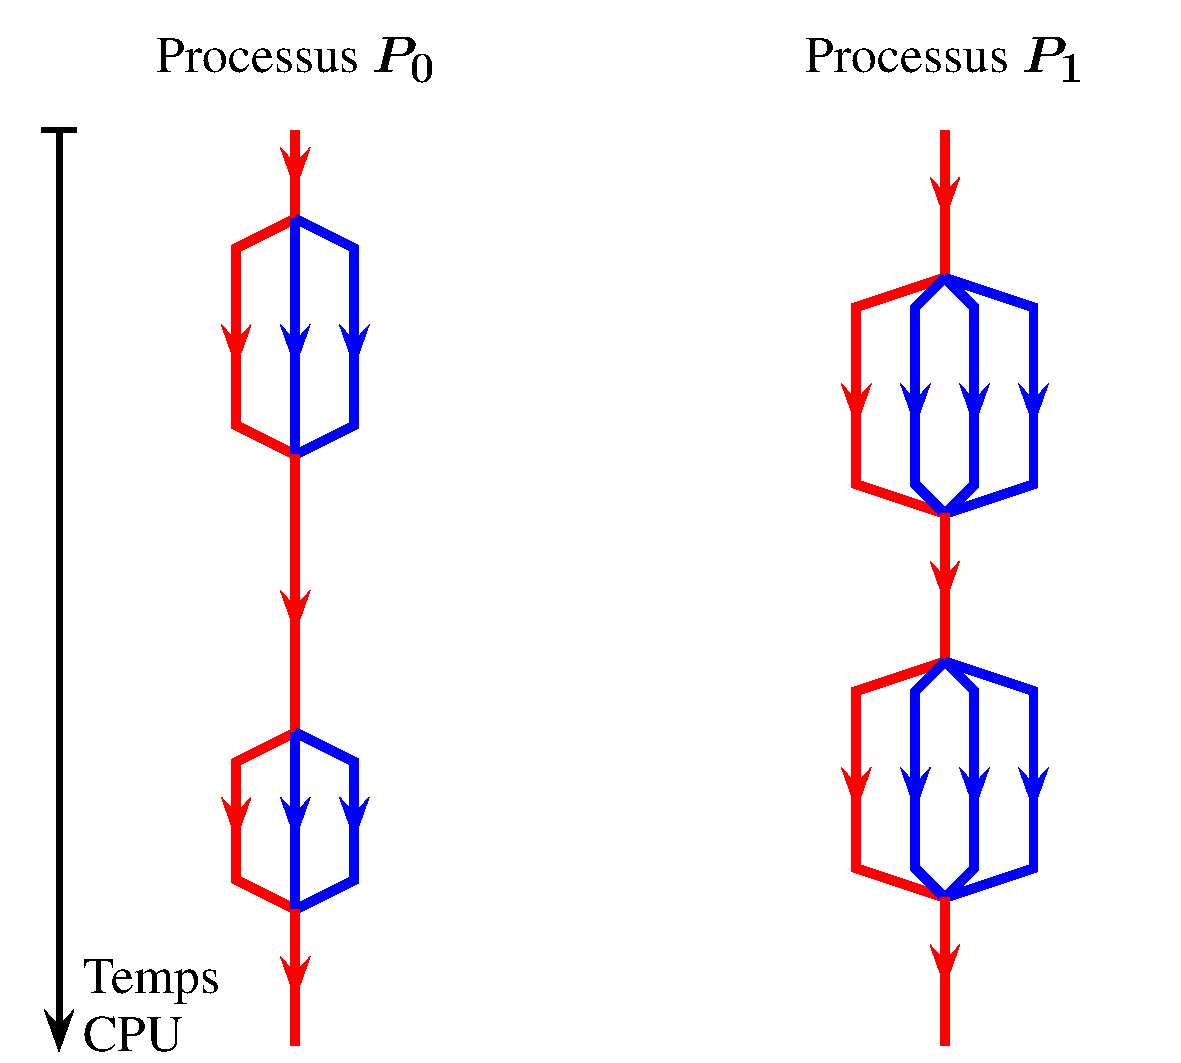
\includegraphics[scale=0.4]{../../Images/enchainementHybride1}
\end{frame}

\begin{frame}
	Quelques types différents de messages
	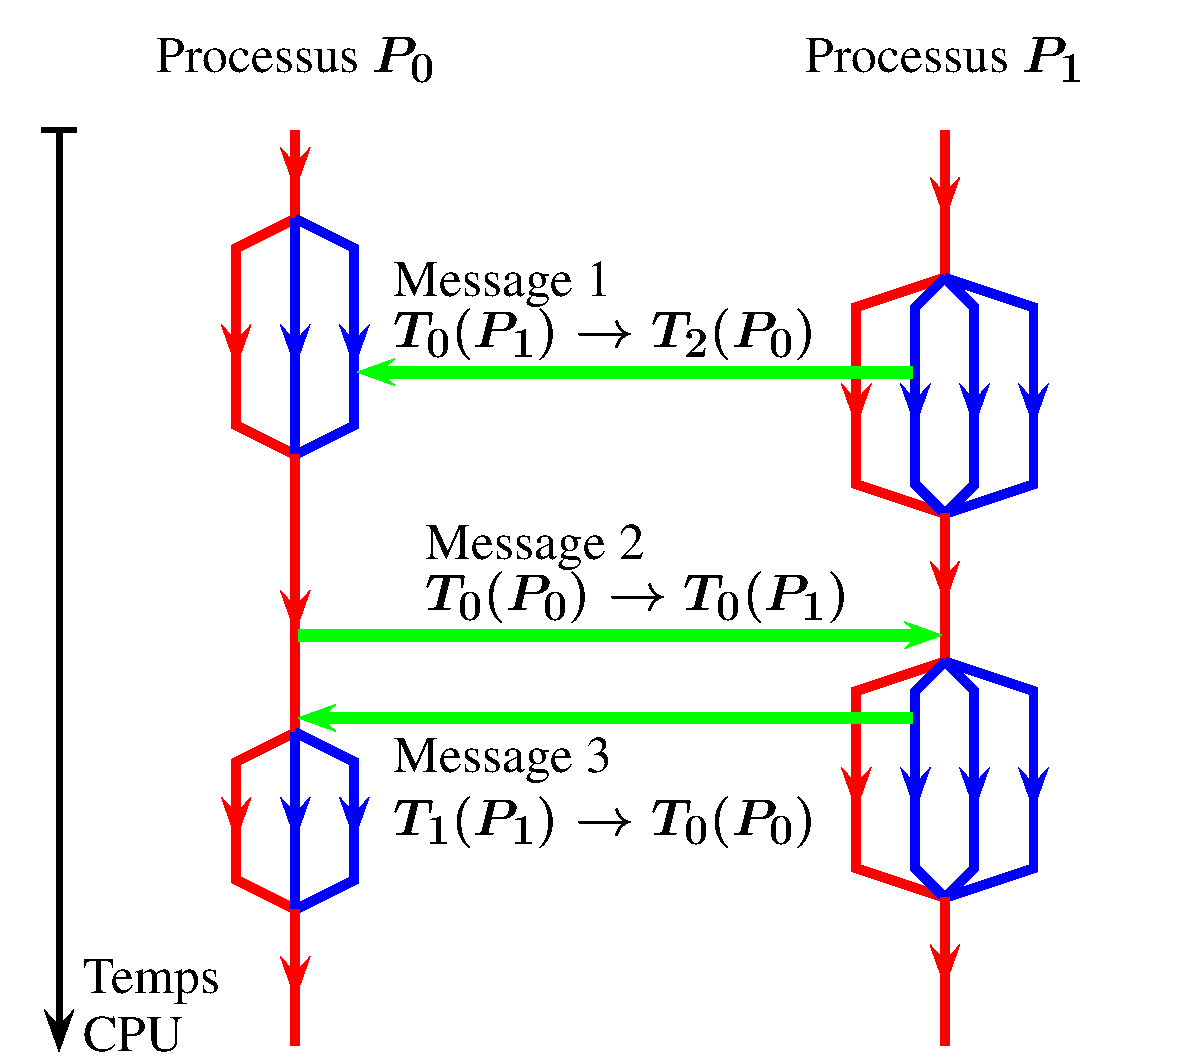
\includegraphics[scale=0.4]{../../Images/enchainementHybride2}
\end{frame}

\begin{frame}
	\vfill
\begin{itemize}
	\item Pas de synchronisation a priori entre les sections multi-threads entre les différents processus, donc besoin éventuel de combiner des barrières OpenMP et MPI
	\vfill
	
	\item 2 types de réductions dans OpenMP et MPI, donc pour faire une réduction complète, il faut combiner ces 2 réductions
	\vfill
	
	\item 2 threads peuvent envoyer chacun un message. Comment  distinguer ces messages (l'ordre d'arrivée est inconnu) ?
	
	\vfill
	\item Si un message arrive dans un processus qui est dans une région multi-threads, quel thread va recevoir et traiter le message ?
\end{itemize}
	\vfill	
	
\end{frame}

\begin{frame}
\vfill
Le grand nombre de situations possibles est très difficile à gérer pour ceux qui développent les libraires OpenMP et MPI

	\vfill
Pour cette raison, 4 niveaux de compatibilité entre OpenMP et MPI, ont été définis:
	\vfill

\begin{itemize}
	\item {\tt\textcolor{blue}{MPI\_THREAD\_SINGLE}}:
	
	Un seul thread par processus (donc pas d'OpenMP)
	\item {\tt\textcolor{blue}{MPI\_THREAD\_FUNNELED}}:
	
	Parmi les threads, seul celui qui a initialisé MPI peut utiliser des fonctions MPI
	\item {\tt\textcolor{blue}{MPI\_THREAD\_SERIALIZED}}:
	
	A un instant donné, un seul thread peut utiliser des fonctions MPI (mais pas toujours le même thread)
	\item {\tt\textcolor{blue}{MPI\_THREAD\_MULTIPLE}}:
	
	Pas de restrictions, tous les threads peuvent utiliser les fonctions MPI.
	
\end{itemize}

\vfill

\end{frame}

\begin{frame}[fragile]
Plus le niveau de compatibilité permet de souplesse dans l'utilisation des fonctions MPI et des pragmas OpenMP, plus la gestion interne des threads dans les processus est coûteuse.

\textcolor{blue}{Donc, il faut choisir le niveau le plus bas suffisant pour l'algorithme du code}

\vfill
Pour choisir le niveau de compatibilité, il faut remplacer
\begin{lstlisting}
MPI_Init(int *argc, char ***argv)
\end{lstlisting}

par
\begin{lstlisting}
MPI_Init_thread(int *argc, char ***argv,
                int required, int *provided)
\end{lstlisting}

\end{frame}

\begin{frame}[fragile]
	où {\tt required} est un entier qui peut prendre une des 4 valeurs \begin{itemize}
		\item {\tt MPI\_THREAD\_SINGLE},
		\item {\tt MPI\_THREAD\_FUNNELED},
		\item {\tt MPI\_THREAD\_SERIALIZED},
		\item {\tt MPI\_THREAD\_MULTIPLE}
	\end{itemize}   
	\vfill
	
	et {\tt provided} est un entier qui reçoit le niveau de compatibilité effectivement proposé par la version de MPI
	
	\vfill
	\textcolor{red}{Il est important de comparer les valeurs de {\tt required} et {\tt provided} pour vérifier que le niveau demandé est effectivement disponible.} 
	
	\vfill
	\textcolor{blue}{{\tt MPI\_Init(...)} est équivalent à {\tt MPI\_Init\_thread(..., MPI\_THREAD\_SINGLE. ...)}}
	
	\vfill
	\texttt{MPI\_Init\_thread} doit être appelé depuis un seul thread (en général le thread 0 dans une région séquentielle pour OpenMP mais
	ce n'est pas obligatoire)
\end{frame}

\begin{frame}
	\vfill
	\textcolor{red}{Dans les cas où plusieurs threads envoient/reçoivent des messages, \textbf{il faut utiliser les tags} pour distinguer ces messages.}
	\bigskip
	
	Sans utiliser le tags, parfois cela marche, parfois non.
	
	\medskip
	Situation analogue aux échanges MPI asynchrones (\texttt{MPI\_Isend/MPI\_Irecv}). D'ailleurs, MPI utilise aussi des threads en interne pour ce type d'échanges.
	\vfill
\end{frame}

\begin{frame}
	Exemples4/Hybrides : différents niveaux de combinaison MPI-OpenMP
	
	\vfill
	
	Remarque:
	\begin{quote}
		Les implémentations de MPI et OpenMP ont fait beaucoup de progrès dans les versions récentes.
		
	\bigskip
		Même si on exécute un code qui utilise un niveau de compatibilité plus élevé que celui demandé dans {\tt MPI\_Init\_thread}, cela peut marcher, mais ce n'est pas garanti.
		
	\bigskip
		Par sécurité, demander un niveau de compatibilité suffisant.
	\end{quote}

	\vfill
	
\end{frame}

\begin{frame}
	
	Suivant les algorithmes du code et d'OpenMP utilisés, on choisira entre les niveaux 
\vfill
	
	\begin{itemize}
		\item \texttt{MPI\_THREAD\_FUNNELED} pour pouvoir faire des appels MPI dans les régions séquentielles d'OpenMP grain fin, ou dans les régions contrôlées par les pragma OpenMP \texttt{MASTER}
		
\vfill
		\item \texttt{MPI\_THREAD\_SERIALIZED} pour pouvoir faire des appels MPI dans les régions contrôlées par les pragma OpenMP \texttt{SINGLE}
		
\vfill
		\item \texttt{MPI\_THREAD\_MULTIPLE} pour pouvoir faire des appels MPI dans les régions parallèles d'OpenMP générales
	\end{itemize}
\vfill

\end{frame}

\begin{frame}[fragile]
	Exemple MPI-OpenMP grain fin
	
\lstset{%
	language={C++},
	breaklines=true,
	captionpos=b,
	basicstyle=\ttfamily,
	numbers=left,
	numbersep=5pt,
	numberstyle=\tiny\color{gray},
	rulecolor=\color{black},
	showspaces=false,
	showstringspaces=false,
	moredelim=[il][\color{red}]{/+},%
}

\begin{lstlisting}{C++}
/+MPI_Init(..., MPI_FUNNELED, ...);
int nX = // nombre de points locaux	
doubl dT, dT_local;
for (iT=0; iT < nT; iT++)
{
  dT_local = calcul_dt(u);
/+  MPI_Allreduce(&dT_local,&dT, ...)
  
/+#pragma omp parallel for
  for (iX=0; iX < nX-1; iX++)
    v[iX]=f(u[iX-1],u[iX],u[iX+1],dT);
    
  echange(u, v);
/+  //echanges MPI sur frontiere locale  
}
	\end{lstlisting}
	
\end{frame}

\begin{frame}[fragile]
Exemple MPI-OpenMP grain grossier
(version 1)

\lstset{%
	language={C++},
	breaklines=true,
	captionpos=b,
	basicstyle=\ttfamily,
	numbers=left,
	numbersep=5pt,
	numberstyle=\tiny\color{gray},
	rulecolor=\color{black},
	showspaces=false,
	showstringspaces=false,
	moredelim=[il][\color{red}]{/+},%
}

\begin{lstlisting}[firstnumber=1]{C++}
/+MPI_Init(..., MPI_FUNNELED, ...);
int nX = // nombre de points locaux (MPI)
 
/+#pragma omp parallel default(shared)
{
  int iT, iX;
  for (iT=0; iT < nT; iT++) {
  
/+#pragma omp master
  {
    dT_local = calcul_dt(u);
/+    MPI_Allreduce(&dT_local, &dT, ...)
  }
/+#pragma omp barrier
  
\end{lstlisting}

\end{frame}
\begin{frame}[fragile]
	Exemple MPI-OpenMP grain grossier (version 1, suite)
	
	\lstset{%
		language={C++},
		breaklines=true,
		captionpos=b,
		basicstyle=\ttfamily,
		numbers=left,
		numbersep=5pt,
		numberstyle=\tiny\color{gray},
		rulecolor=\color{black},
		showspaces=false,
		showstringspaces=false,
		moredelim=[il][\color{red}]{/+},%
	}
	
\begin{lstlisting}[firstnumber=15]{C++}
  /+#pragma omp for
  for (iX=1; iX < nX-1; iX++)
    v[iX] = f(u[iX-1],u[iX],u[iX+1],dT)

  /+#pragma omp master
  {
    echange(u, v);
/+    //echanges MPI sur frontiere locale    
  }
}
\end{lstlisting}

\end{frame}
\begin{frame}[fragile]
	Exemple MPI-OpenMP grain grossier (version 2)
	
	\lstset{%
		language={C++},
		breaklines=true,
		captionpos=b,
		basicstyle=\ttfamily,
		numbers=left,
		numbersep=5pt,
		numberstyle=\tiny\color{gray},
		rulecolor=\color{black},
		showspaces=false,
		showstringspaces=false,
		moredelim=[il][\color{red}]{/+},%
	}
	
	\begin{lstlisting}[firstnumber=1]{C++}
/+MPI_Init(..., MPI_SERIALIZED, ...);
int nX = // nombre de points locaux (MPI)
	
/+#pragma omp parallel default(shared)
{
  int iT, iX;
  for (iT=0; iT < nT; iT++) {

  /+#pragma omp single
  {
    dT_local = calcul_dt(u);
  /+  MPI_Allreduce(&dT_local, &dT, ...)
  }
	
\end{lstlisting}
	
\end{frame}
\begin{frame}[fragile]
	Exemple MPI-OpenMP grain grossier (version 2, suite)
	
	\lstset{%
		language={C++},
		breaklines=true,
		captionpos=b,
		basicstyle=\ttfamily,
		numbers=left,
		numbersep=5pt,
		numberstyle=\tiny\color{gray},
		rulecolor=\color{black},
		showspaces=false,
		showstringspaces=false,
		moredelim=[il][\color{red}]{/+},%
	}
	
	\begin{lstlisting}[firstnumber=14]{C++}
	
  /+#pragma omp for
  for (iX=1; iX < nX-1; iX++)
    v[iX] = f(u[iX-1],u[iX],u[iX+1],dT)

  /+#pragma omp single
  {
    echange(u, v);
    /+// echanges MPI sur frontiere locale    
  }
}
\end{lstlisting}
	
\end{frame}

\begin{frame}
	Les appels MPI globaux (\texttt{MPI\_Reduce}, \texttt{MPI\_Gather}, etc)
	doivent être faits dans un seul thread par processus (celui qui a appelé \texttt{MPI\_Init\_thread}).
	
	\bigskip
	En général, les appels sont faits dans les parties séquentielles (au sens OpenMP) ou dans les parties des régions OpenMP parallèles contrôlées par les \texttt{pragma omp master}. 
\end{frame}

\begin{frame}
Exemple4/PoissonMPI : code MPI auquel est ajoutée une parallélisation OpenMP grain fin
\end{frame}
\end{document}
